\pdfoutput=1
\documentclass[11pt]{article}

\usepackage[letterpaper,margin=1in]{geometry}
\usepackage[T1]{fontenc}
\usepackage[utf8]{inputenc}
\usepackage{lmodern}
\usepackage{microtype}
\usepackage{amsmath,amssymb}
\usepackage{booktabs}
\usepackage{graphicx}
\usepackage{url}
\usepackage[numbers]{natbib}
\usepackage{algorithm}
\usepackage{algpseudocode}
\usepackage{enumitem}
\usepackage{array}
\usepackage{float}
\usepackage{xcolor}
\usepackage{authblk}
\usepackage{abstract}
\usepackage{caption}
\usepackage{titlesec}
\usepackage{fancyhdr}
\usepackage{hyperref}

\graphicspath{{./figures/}}

\definecolor{arxivblue}{HTML}{1F4E79}
\definecolor{darkgray}{HTML}{333333}

\hypersetup{
  colorlinks=true,
  linkcolor=arxivblue,
  citecolor=arxivblue,
  urlcolor=arxivblue,
  pdfauthor={ScoreSG authors},
  pdftitle={ScoreSG: Scalable Anti-Hub Support Graphs for Density Hierarchies}
}
\urlstyle{same}

\pagestyle{fancy}
\fancyhf{}
\lhead{\small ScoreSG}
\rhead{\small arXiv preprint}
\cfoot{\thepage}
\setlength{\headheight}{14pt}
\renewcommand{\headrulewidth}{0.4pt}

\titleformat{\section}
  {\large\bfseries\color{darkgray}}
  {\thesection}{0.75em}{}
\titleformat{\subsection}
  {\normalsize\bfseries\color{darkgray}}
  {\thesubsection}{0.75em}{}
\titleformat{\paragraph}[runin]
  {\bfseries}
  {}{0pt}{}
\titlespacing*{\section}{0pt}{2.0ex plus 0.5ex minus 0.2ex}{1.0ex}
\titlespacing*{\subsection}{0pt}{1.5ex plus 0.4ex minus 0.2ex}{0.7ex}
\titlespacing*{\paragraph}{0pt}{1.0ex}{0.5em}

\renewcommand{\abstractnamefont}{\normalfont\bfseries}
\renewcommand{\abstracttextfont}{\normalfont\small}
\setlength{\absleftindent}{0.06\textwidth}
\setlength{\absrightindent}{0.06\textwidth}
\captionsetup{font=small,labelfont=bf}
\setlist[itemize]{leftmargin=*,topsep=0.35em,itemsep=0.15em}

\newcommand{\keywords}[1]{%
  \vspace{0.75em}
  \begin{center}
  \begin{minipage}{0.88\textwidth}
  \small\noindent\textbf{Keywords:} #1
  \end{minipage}
  \end{center}
}

\title{\textbf{ScoreSG: Scalable Anti-Hub Support Graphs for Density Hierarchies}\\
\large Sparse Approximate Support Graphs for Repeated Multi-\(k\) HDBSCAN-Style Workflows}

\author{}

\date{\small September 2026}

\begin{document}
\maketitle

\begin{abstract}
Hierarchical density-based clustering is often used in exploratory settings where several neighborhood-parameter values must be evaluated on the same dataset. HDBSCAN constructs a hierarchy from mutual-reachability distances, but repeated execution across many values of \(k\) can make multi-resolution analysis computationally expensive. CoreSG reduces this cost by reusing a support graph for multiple minimum-spanning-tree extractions, although its exact construction still relies on dense pairwise distance information. We present ScoreSG, a sparse approximate construction for CoreSG that combines approximate \(k\)-nearest-neighbor discovery with anti-hub reinforcement. ScoreSG builds an approximate directed \(k_{\max}\)-nearest-neighbor graph with PyNNDescent, estimates core-distance lists from this graph, selects \(\lfloor\sqrt{N}\rfloor\) low in-degree vertices as anti-hubs, and adds exact-distance clique edges among them before reusing the CoreSG reweighting, MST extraction, and hierarchy pipeline. We first evaluate support-graph connectivity over 405 separated-cluster synthetic configurations with up to \(10^6\) samples and 128 dimensions. The stress-test grid uses six cluster centers, center separation 10.0, within-cluster scale 0.3, nine marginal noise distributions, and seed 42. The ScoreSG support graph was connected in 398 configurations for all 49 requested \(k\) values; a random \(\sqrt{N}\)-clique baseline was also connected in 398, whereas the approximate \(k\)NN-only support was connected in none. These results show that sparse reinforcement often restores the minimum condition needed for MST extraction in separated-cluster supports, although connectivity is not equivalent to recovering complete-graph MST edges. We then evaluate cumulative runtime on synthetic Gaussian-mixture benchmarks with 20 features, 10 centers, \(k \in \{50,\ldots,2\}\), and 30 timing repetitions per configuration. At \(N=50{,}000\), ScoreSG completes the full workflow in 224.36 s, compared with 525.45 s for CoreSG, 1342.44 s for Optimized HDBSCAN, and 9272.92 s for HDBSCAN. In the Gaussian quality benchmark, ScoreSG completes all 1960 requested \(k\) evaluations with mean ARI 0.9015 against generic HDBSCAN, mean HAI 0.9738, and mean workflow time 87.70 s.
\end{abstract}
\keywords{density-based clustering; HDBSCAN; support graphs; approximate nearest neighbors; anti-hubs; minimum spanning trees; multi-\(k\) analysis}

\section{Introduction}

\subsection{The Problem}

Density-based clustering is designed for data in which clusters may have irregular geometry, heterogeneous density, and noise. HDBSCAN is widely used because it replaces a single density threshold with a hierarchy induced by mutual-reachability distances and then selects clusters through stability criteria \citep{campello2013density,campello2015hierarchical}. This hierarchy is especially useful in exploratory analysis, where the goal is usually not to inspect a single partition. Instead, analysts typically compare a sequence of results across density scales, neighborhood parameters, or cluster granularities before deciding which structure is scientifically or operationally meaningful.

The computational question studied in this paper is therefore not the cost of a single clustering run. It is the cumulative cost of obtaining a sequence of HDBSCAN-style hierarchy outputs for \(K=\{2,\ldots,k_{\max}\}\) on the same input dataset. Standard HDBSCAN execution repeats the main computation for each parameter value. CoreSG changes this regime by constructing a reusable support graph and extracting multiple MSTs from it \citep{araujo2022coresg}. The gain is structural: when the analyst needs many related outputs, the construction cost can be incurred once and amortized over the sequence of extractions. However, the exact CoreSG path still requires dense pairwise distance information, which limits scalability as \(N\) grows.

\subsection{Approach and Contributions}

ScoreSG addresses this bottleneck with a sparse approximate support graph. The method begins with an approximate \(k_{\max}\)-nearest-neighbor graph built by PyNNDescent, a Python implementation inspired by NN-Descent \citep{dong2011efficient,pynndescentdocs}. It then identifies anti-hubs, namely points that rarely appear in other points' directed neighbor lists, and connects a subset of size \(\lfloor\sqrt{N}\rfloor\) with exact-distance clique edges. The clique is quadratic only in the number of selected anti-hubs, so its edge count is linear in \(N\). Downstream, ScoreSG reuses the same mutual-reachability reweighting, MST extraction, and hierarchy conversion used by CoreSG.

The central observation is that sparse neighbor graphs can omit edges needed by the complete-graph MST. These missing edges matter because HDBSCAN-style hierarchies depend on an MST over mutual-reachability distances. In this paper, connectivity is treated as a prerequisite rather than as evidence of exact recovery: a connected support graph can still miss MST edges, while a disconnected support graph cannot produce any spanning tree. ScoreSG does not claim to recover all missing edges. Instead, it introduces a scalable reinforcement mechanism that increases support among low in-degree points while preserving sparsity. If the resulting support graph is disconnected, ScoreSG fails explicitly rather than silently injecting exact MST edges.

The contribution of ScoreSG is therefore both algorithmic and practical. Algorithmically, it replaces the dense construction bottleneck with a sparse approximate support and a linear-edge reinforcement strategy for low in-degree vertices. This provides a graph-construction route for repeated HDBSCAN-style hierarchy extraction without making exact MST-edge recovery part of the method definition. From a usability perspective, ScoreSG preserves the reusable CoreSG workflow: the support is built once for \(k_{\max}\), and the user can inspect a sequence of hierarchy outputs over multiple \(k\) values without launching independent clustering runs for each parameter.

This paper makes four contributions. We introduce ScoreSG, a sparse approximate construction for reusable HDBSCAN-style hierarchy extraction, demonstrated by a concrete implementation in the BSD-3-Clause Python package \texttt{core-sg}. We formalize anti-hub reinforcement as a linear-edge augmentation strategy for sparse support graphs, in contrast to dense complete-graph repair. We also evaluate the structural premise through support-graph connectivity diagnostics on separated-cluster synthetic stress tests, including a random \(\sqrt{N}\)-clique baseline that separates the effect of sparse clique reinforcement from the effect of the specific anti-hub ranking. Finally, we evaluate cumulative runtime, partition agreement, and hierarchy agreement in repeated multi-\(k\) workflows.

\subsection{Research Questions}

The study is organized around four research questions:
\begin{description}[leftmargin=*,font=\normalfont\bfseries]
  \item[RQ1.] Can sparse anti-hub reinforcement restore the minimum connectivity condition required for MST extraction in separated-cluster support graphs?
  \item[RQ2.] How does ScoreSG change cumulative runtime in repeated multi-\(k\) HDBSCAN-style workflows?
  \item[RQ3.] How closely do ScoreSG outputs agree with HDBSCAN-style references in partition and hierarchy quality?
  \item[RQ4.] Does anti-hub selection provide evidence beyond random sparse clique reinforcement in the reported diagnostics?
\end{description}

\subsection{Paper Organization}

Section~\ref{sec:related-work} reviews density-based hierarchy construction, reusable MST computation, approximate neighbor search, and quality evaluation. Section~\ref{sec:preliminaries} defines the graph objects and cumulative-runtime objective. Section~\ref{sec:method} presents ScoreSG. Section~\ref{sec:diagnostics} reports structural diagnostics and ablations. Section~\ref{sec:experimental-setup} describes the datasets, methods, and metrics. Section~\ref{sec:results} reports runtime and quality results. Section~\ref{sec:discussion} discusses implications and limitations.

\section{Related Work}
\label{sec:related-work}

\paragraph{Density-based hierarchical clustering.}
HDBSCAN constructs a density hierarchy from mutual-reachability distances and then extracts stable clusters from that hierarchy \citep{campello2013density,campello2015hierarchical}. Its main advantage over flat density clustering is that it represents structure across density levels rather than requiring a single global density threshold. This makes it useful in applications where clusters are non-convex, have different densities, or coexist with noise. The relevant disadvantage is computational: when a user wants to compare many neighborhood parameters, HDBSCAN is typically executed repeatedly, and each execution incurs the cost of neighbor search, graph construction, MST construction, and hierarchy extraction for that particular parameter.

\paragraph{Optimized HDBSCAN implementations.}
The scikit-learn-contrib implementation associated with Leland McInnes and collaborators introduced practical accelerations and exposes an \texttt{algorithm="best"} mode that selects an optimized internal strategy when possible \citep{mcinnes2017accelerated,hdbscansoftware}. This implementation is the baseline called Optimized HDBSCAN in our experiments. It is a strong practical baseline because it represents the implementation a Python user is likely to choose for scalable HDBSCAN-style clustering. Its advantage is efficient single-run execution through implementation-level algorithm selection. Its limitation in this setting is that it still treats different \(k\) values as separate clustering runs. The baseline called HDBSCAN uses the same HDBSCAN objective with the generic internal algorithm and represents the non-specialized execution path.

\paragraph{Reusable MST computation and CoreSG.}
CoreSG was introduced to compute multiple MSTs for density-based methods by reusing a graph support structure across a range of \(k\) values \citep{araujo2022coresg}. This directly matches the exploratory setting in which analysts inspect not one output, but a sequence of clusterings or hierarchies. CoreSG's advantage is amortization: once the support is built for \(k_{\max}\), the method can reweight and extract MSTs for smaller \(k\) values without repeating the full HDBSCAN computation. This makes CoreSG the natural exact reusable baseline for ScoreSG. However, its exact construction path still depends on dense pairwise information, which creates a practical scalability barrier as \(N\) increases.

\paragraph{Approximate nearest-neighbor graph construction.}
Approximate \(k\)-nearest-neighbor graph construction reduces the cost of identifying candidate local neighborhoods in large datasets. NN-Descent is a representative method for generic similarity measures \citep{dong2011efficient}, and PyNNDescent provides the implementation used by ScoreSG \citep{pynndescentdocs}. Approximate neighbor search avoids explicit all-pairs distance computation and produces sparse candidate edges. However, approximate neighbor membership is not an exact certificate: relevant edges may be absent, and the resulting graph can be disconnected or can induce an MST different from the complete mutual-reachability MST.

\paragraph{Missing edges and sparse support graphs.}
Sparse graph construction introduces a tension between computational efficiency and graph sufficiency. A \(k\)NN graph may contain enough local edges for many clustering tasks, but HDBSCAN-style hierarchy construction depends on an MST. If the sparse support omits complete-graph MST edges, exact recovery is no longer guaranteed. Increasing \(k\) can reduce this risk, but it increases graph size and does not by itself guarantee connectivity for every data geometry. Adding dense repair edges can solve connectivity, but it reintroduces the computational behavior that the sparse method seeks to avoid. ScoreSG positions anti-hub reinforcement between these extremes: it adds targeted support to low in-degree vertices while keeping the number of added clique edges linear in \(N\).

\paragraph{Partition- and hierarchy-quality evaluation.}
Runtime alone is insufficient for an approximate clustering method. When ground-truth or reference labels are available, the Adjusted Rand Index (ARI) is a standard external measure for comparing a predicted partition with a reference partition while correcting for chance agreement \citep{hubert1985comparing}. In this paper, ARI is the partition-quality axis used to compare the flat clustering labels extracted at each value of \(k\).

Hierarchy-level agreement is also required because two methods may produce similar flat partitions at a selected \(k\) while differing in the hierarchies from which those partitions were extracted. We therefore use the Hierarchy Agreement Index (HAI), proposed by \citet{johnson2013comprehensive}, to compare hierarchy structure. HAI extends the pairwise logic of the Rand Index to hierarchical clustering by comparing, for each pair of points, how closely the two hierarchies place that pair in their smallest shared cluster. This makes it suitable for evaluating whether an approximate support graph preserves the density hierarchy induced by an exact reference, rather than only a selected flat partition. The same pairwise hierarchy-similarity principle has also been used to analyze collections of HDBSCAN* hierarchies over multiple \texttt{mpts} values.

\paragraph{Positioning of ScoreSG.}
ScoreSG is neither a new density-cluster selection rule nor a replacement for HDBSCAN in all settings. It is a graph-construction method for repeated HDBSCAN-style hierarchy extraction. Its scientific claim is about computational scalability under a multi-\(k\) workflow, where the relevant object is a sequence of results rather than a single partition. The quality evaluation reported in this paper measures partition and hierarchy agreement against HDBSCAN-style references on the tested Gaussian synthetic grid.

\section{Preliminaries and Problem Formulation}
\label{sec:preliminaries}

Let \(X=\{x_i\}_{i=1}^{N}\), with \(x_i \in \mathbb{R}^{d}\), and let \(d(x_i,x_j)\) be a metric distance. For a neighborhood parameter \(k\), the core distance \(c_k(i)\) is the distance from \(x_i\) to its \(k\)-th nearest neighbor. The mutual-reachability distance between two points is
\begin{equation}
  w_k(i,j) = \max\{c_k(i), c_k(j), d(x_i,x_j)\}.
\end{equation}
HDBSCAN-style hierarchy construction can be expressed as an MST over a graph weighted by \(w_k\), followed by hierarchy construction and stability-based cluster extraction \citep{campello2015hierarchical}.

Let \(G^c_k=(V,E^c,w_k)\) be the complete mutual-reachability graph and let \(T^c_k\) be an MST of \(G^c_k\). A sparse support graph \(G^s=(V,E^s)\) is sufficient for exact MST recovery at \(k\) only if it contains at least one complete-graph MST:
\begin{equation}
  E(T^c_k) \subseteq E^s.
\end{equation}
A missing edge is therefore an edge \(e \in E(T^c_k)\) that is absent from \(E^s\). If such an edge is absent, then no MST extracted from \(G^s\) can equal that particular \(T^c_k\). If \(G^s\) is disconnected, no spanning tree exists in \(G^s\). The two conditions are related but not equivalent: connectivity is necessary for MST extraction, whereas missing-edge recovery requires the support to contain the MST edges selected by the complete mutual-reachability graph. This paper measures connectivity as a structural prerequisite rather than as a direct MST-edge recall measure.

The optimization objective evaluated in this paper is cumulative runtime over multiple \(k\) values. For reusable methods,
\begin{equation}
  T_{\mathrm{reuse}}(N) = T_{\mathrm{build}}(N,k_{\max}) + \sum_{k=2}^{k_{\max}} T_{\mathrm{extract}}(N,k).
\end{equation}
For methods that are rerun independently,
\begin{equation}
  T_{\mathrm{rerun}}(N) = \sum_{k=2}^{k_{\max}} T_{\mathrm{fit}}(N,k).
\end{equation}
This distinction is essential: a method optimized for a single \(k\) may be inefficient when the analysis requires dozens of related hierarchy extractions.

\section{Method: ScoreSG}
\label{sec:method}

\subsection{Construction Pipeline}

Figure~\ref{fig:coresg-overview} shows the exact CoreSG workflow: pairwise distances are computed, a \(k\)NN graph and CoreSG support are built, and the support is reweighted for each requested \(k\) before MST and hierarchy extraction. Figure~\ref{fig:scoresg-pipeline} shows the ScoreSG replacement for the construction stage.

\begin{figure}[H]
\centering
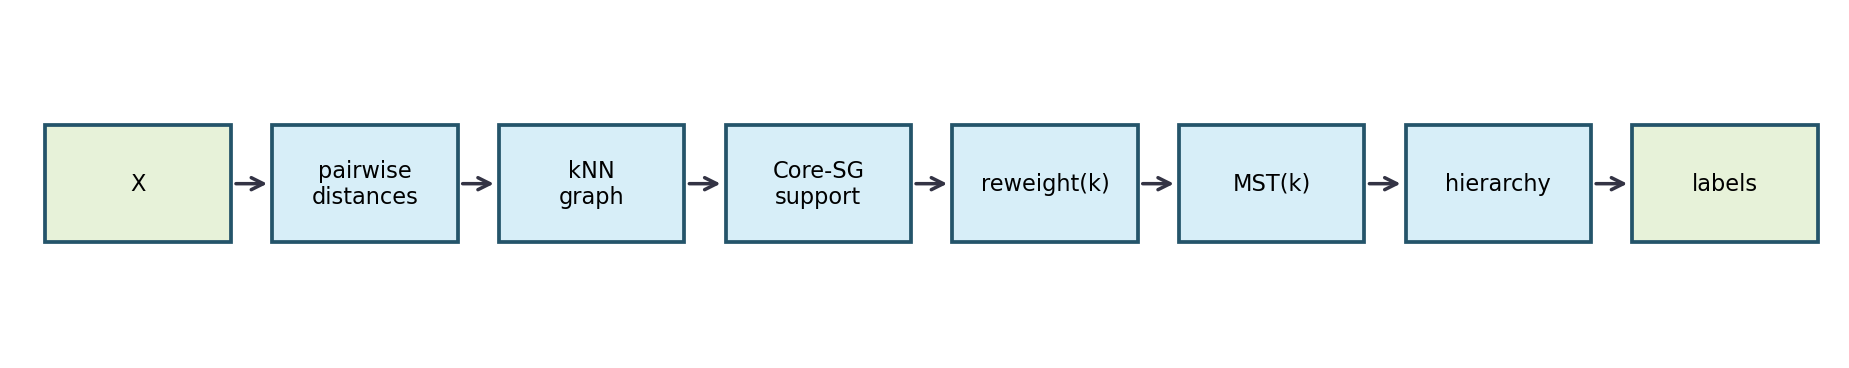
\includegraphics[width=\linewidth,keepaspectratio]{pipeline_overview.png}
\caption{Exact CoreSG pipeline. The reusable workflow builds support once and then reweights and extracts MST-based hierarchies for different \(k\) values.}
\label{fig:coresg-overview}
\end{figure}

\begin{figure}[H]
\centering
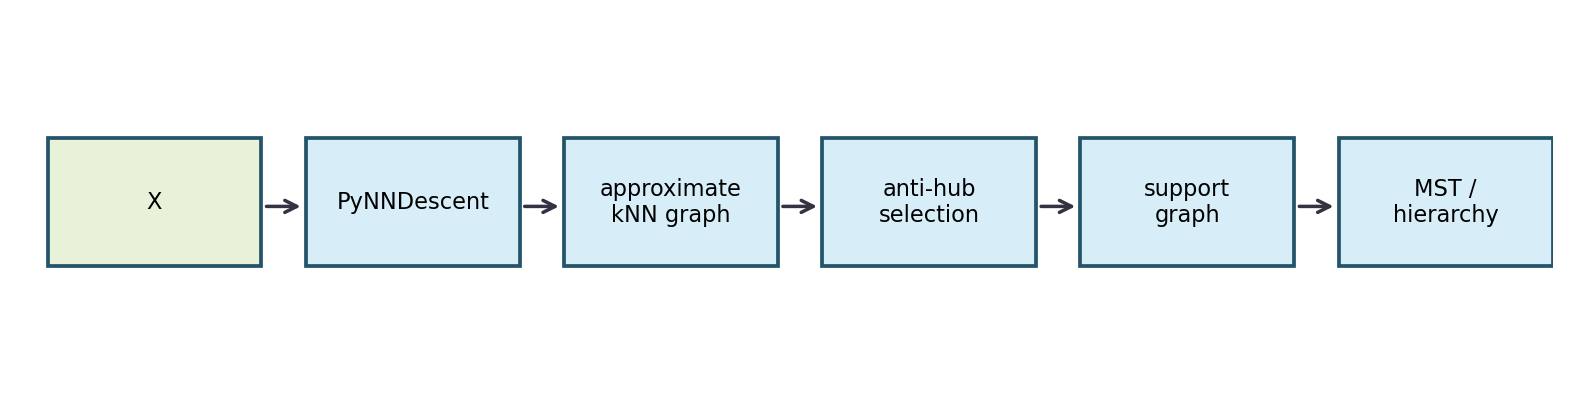
\includegraphics[width=\linewidth,keepaspectratio]{score_sg_pipeline.png}
\caption{ScoreSG pipeline. Pairwise dense construction is replaced by approximate neighbor discovery, anti-hub selection, sparse support reinforcement, and the same MST/hierarchy extraction stage used by CoreSG.}
\label{fig:scoresg-pipeline}
\end{figure}

ScoreSG has five stages. PyNNDescent builds an approximate directed \(k_{\max}\)-nearest-neighbor graph; each neighbor list is then normalized by removing self-neighbors and sorting by approximate distance. Core-distance lists are estimated from these neighbor distances, vertices are scored by directed in-degree, and anti-hubs are selected. Finally, exact distances are computed only for selected support edges: approximate \(k\)NN edges and clique edges among selected anti-hubs.

\subsection{Anti-Hub Reinforcement}

Let \(A(i)\) be the directed approximate neighbor list of \(x_i\). The directed in-degree of vertex \(j\) is
\begin{equation}
  \deg^{-}(j)=|\{i: j \in A(i)\}|.
\end{equation}
A low value of \(\deg^{-}(j)\) indicates that \(x_j\) is rarely chosen as a neighbor by other points. ScoreSG selects
\begin{equation}
  m=\max(1,\lfloor\sqrt{N}\rfloor)
\end{equation}
vertices with lowest directed in-degree. Ties are resolved by the sum of in-degrees of each candidate's outgoing neighbors, followed by seeded random tie-breaking when needed. The selected vertices are connected as a clique with exact metric distances.

The clique size is
\begin{equation}
  |E_{\mathrm{anti\text{-}hub}}|=\frac{m(m-1)}{2}=O(N),
\end{equation}
because \(m=O(\sqrt{N})\). Thus, anti-hub reinforcement is dense inside the selected subset but linear in the full dataset size. This design targets disconnected sparse supports and the risk of omitted MST edges while avoiding complete-graph construction. Algorithm~\ref{alg:scoresg} summarizes the construction.

\begin{algorithm}[H]
\caption{ScoreSG support-graph construction}
\label{alg:scoresg}
\begin{algorithmic}[1]
\Require Dataset \(X\), maximum neighborhood \(k_{\max}\), metric \(d\), random state \(s\)
\State Build approximate directed \(k_{\max}\)NN graph \(A\) using PyNNDescent.
\State Remove self-neighbors and sort each outgoing list by distance.
\State Estimate core-distance lists from approximate neighbor distances.
\State Compute \(\deg^{-}(j)\) for each vertex \(j\).
\State Select \(m=\max(1,\lfloor\sqrt{N}\rfloor)\) vertices with smallest \(\deg^{-}\).
\State Compute exact distances for all approximate \(k\)NN support edges.
\State Add exact-distance clique edges among selected anti-hubs.
\State Return the sparse support graph for CoreSG reweighting and MST extraction.
\end{algorithmic}
\end{algorithm}

\subsection{Complexity}

The exact CoreSG path constructs dense pairwise information, which requires \(O(N^2)\) memory or distance evaluations when materialized. ScoreSG avoids this explicit dense stage. Its support graph contains approximately \(Nk_{\max}\) approximate neighbor edges plus \(O(N)\) anti-hub clique edges. Reweighting and MST extraction then operate on this sparse support. Under the intended operating regime \(k_{\max} \ll N\), the support size grows approximately linearly in \(N\) for fixed \(k_{\max}\), up to approximate-neighbor search overhead and sorting. Therefore, the main scalability claim is sparse scaling of the constructed support graph, not a formal end-to-end linear-time proof for every backend operation.

\subsection{Failure Semantics}

ScoreSG checks whether the constructed support graph is connected before MST extraction. If it is disconnected, the method raises an explicit error. This behavior is deliberate: a disconnected support graph cannot support a spanning tree, and silently adding complete-graph MST edges would invalidate the sparse construction claim.

\section{Structural Diagnostics and Ablation Study}
\label{sec:diagnostics}

\subsection{Tie-Aware Anti-Hub Selection}
\label{sec:tie-aware-missing-edge}

The anti-hub procedure is used as a sparse mechanism for proposing edges that may compensate for omissions in the approximate \(k\)NN support. It does not enumerate the missing edges of the complete mutual-reachability MST, because doing so would require constructing the object that ScoreSG is designed to avoid. Instead, it searches for low in-degree vertices that are likely to lie outside dense hub regions and then connects a controlled subset of them.

A direct ranking by in-degree is not sufficient when many vertices share the same in-degree at the selection boundary. If all selected anti-hubs are drawn from a tied group, the procedure moves toward random selection. ScoreSG therefore uses a secondary score for tied candidates:
\begin{equation}
  s(j)=\sum_{u\in A(j)} \deg^{-}(u).
\end{equation}
Lower values of \(s(j)\) indicate that the candidate is connected to a low-degree neighborhood and is therefore preferred during tie-breaking.

We evaluate this tie behavior on a separated-cluster synthetic diagnostic grid. The grid uses the nine distributions in Table~\ref{tab:missing-edge-distributions}, nine sample sizes \(N\in\{1{,}000,5{,}000,10{,}000,25{,}000,50{,}000,100{,}000,200{,}000,500{,}000,1{,}000{,}000\}\), five dimensions \(d\in\{2,10,32,64,128\}\), and seed 42. For each base distribution, the generator standardizes a distributional draw and uses it as local noise around six separated centers. The final reported stress test uses center separation 10.0 and within-cluster scale 0.3, producing compact clusters with sparse regions between groups. This setting stresses the structural support problem: when clusters are well separated, a local approximate \(k\)NN graph can remain disconnected even when each individual cluster is internally well represented.

\begin{table}[H]
\centering
\caption{Synthetic distributions used in the missing-edge and connectivity diagnostics. Parameters are the values used by the experiment script.}
\label{tab:missing-edge-distributions}
\resizebox{\linewidth}{!}{
\begin{tabular}{lll}
\toprule
Distribution & Generation parameters & Diagnostic role \\
\midrule
Gaussian & \(\mathcal{N}(0,1)\) independently per feature & Continuous symmetric baseline \\
Poisson & \(\lambda=5\) independently per feature & Discrete count-valued data \\
Chi-square & \(\chi^2\) with 2 degrees of freedom & Positive skewed continuous data \\
Gamma & Shape 2.0, scale 2.0 & Positive skewed continuous data \\
Beta & \(a=2.0,b=5.0\) & Bounded continuous data \\
Von Mises & \(\mu=0,\kappa=4.0\) & Concentrated angular-valued samples used as Euclidean features \\
Gumbel & Location 0.0, scale 1.0 & Asymmetric extreme-value distribution \\
Logistic & Location 0.0, scale 1.0 & Heavy-tailed continuous distribution \\
Gaussian sparse label & \(\mathcal{N}(0,1)\); zero insertion disabled in the final separated-cluster run & Compatibility control retained from the sparse-grid script \\
\bottomrule
\end{tabular}
}
\end{table}

The tie diagnostic compares two quantities: the number of selected anti-hubs that would still be chosen from the boundary degree-tie group under degree-only ranking, and the number that remains tied after applying the secondary score. Table~\ref{tab:tie-breaking} and Figure~\ref{fig:ties} show that, on the final separated-cluster grid, the score reduces the mean number of still-tied selected anti-hubs from 337.17 to 1.14 at \(d=128\). This result supports the score as a deterministic anti-hub selection step, but it does not by itself establish MST-edge recovery or clustering-quality equivalence.

\begin{table}[H]
\centering
\caption{Tie behavior in anti-hub selection over the final separated-cluster synthetic connectivity grid. Values are means across 81 configurations per dimension: nine distributions and nine sample sizes.}
\label{tab:tie-breaking}
\resizebox{\linewidth}{!}{
\begin{tabular}{rrrrr}
\toprule
Dimensions & Configurations & Tied candidates before score & Selected from ties, degree only & Selected from ties, score tie-break \\
\midrule
2 & 81 & 13715.67 & 57.84 & 4.68 \\
10 & 81 & 324.91 & 98.53 & 1.20 \\
32 & 81 & 3858.84 & 329.53 & 1.36 \\
64 & 81 & 13142.54 & 335.02 & 1.28 \\
128 & 81 & 32239.28 & 337.17 & 1.14 \\
\bottomrule
\end{tabular}
}
\end{table}

\begin{figure}[H]
\centering
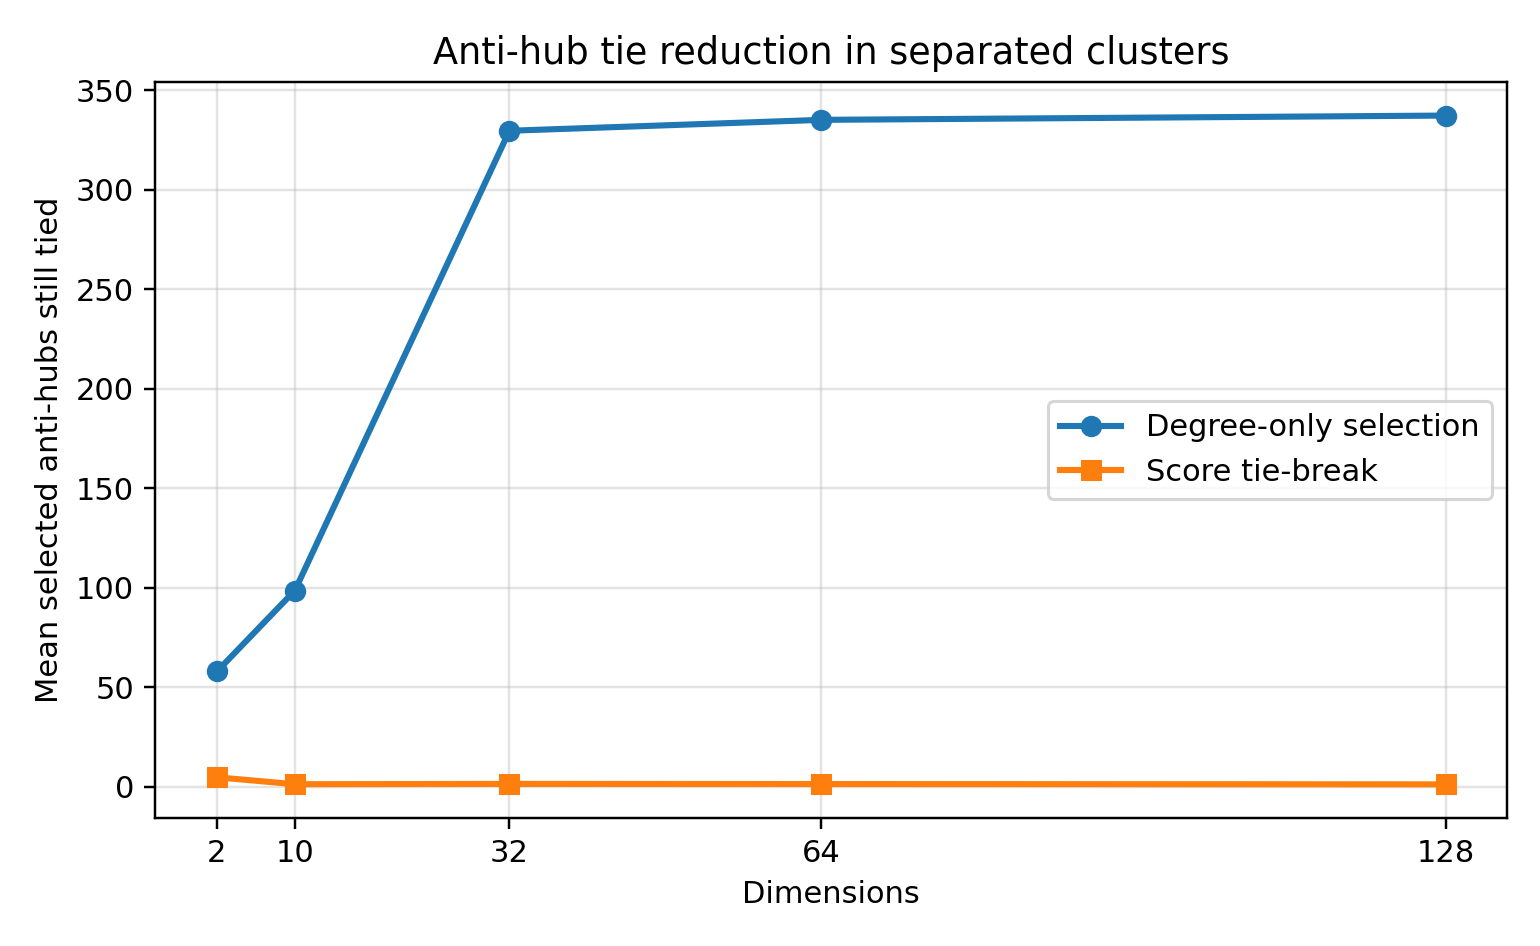
\includegraphics[width=0.74\linewidth,keepaspectratio]{score_sg_tie_break_by_dimension.png}
\caption{Mean number of selected anti-hubs that remain tied before and after the secondary score, aggregated by dimension over the final separated-cluster synthetic connectivity grid. The score-based tie-break reduces random boundary selection across all tested dimensions.}
\label{fig:ties}
\end{figure}

\subsection{Connectivity as a Minimum Structural Diagnostic}

ScoreSG requires a graph-validity diagnostic because MST extraction is defined only on connected support graphs. The connectivity test evaluates whether the sparse support graph constructed from approximate neighbors and reinforcement edges contains a single connected component before hierarchy extraction. This test is deliberately weaker than a missing-edge recall experiment. Connectivity verifies the minimum structural condition required for MST extraction; missing-edge recovery would require checking whether the support contains the MST edges of the complete mutual-reachability graph.

The connectivity diagnostic uses the final separated-cluster synthetic grid described in Section~\ref{sec:tie-aware-missing-edge}. It contains 405 configurations: nine marginal noise distributions, nine sample sizes, five dimensions, six separated centers, center separation 10.0, within-cluster scale 0.3, and seed 42. For each dataset, we build a reusable support at \(k_{\max}=50\) and verify connectivity for the 49 requested values \(k=50,49,\ldots,2\). Because the reusable support does not change across these extractions, each connected support contributes 49 connected checks.

We compare three support variants. The first is the approximate \(k\)NN graph without reinforcement. The second is a random baseline that selects \(\lfloor\sqrt{N}\rfloor\) vertices uniformly at random and adds the same exact-distance clique used by ScoreSG. The third is ScoreSG, which selects the same number of vertices by low in-degree with the score-based tie-breaking rule. The random baseline controls for whether connectivity gains arise simply from adding an \(O(N)\)-edge clique or from the specific anti-hub ranking. It is not a missing-edge recovery baseline: a random clique can connect components while still omitting edges that would appear in the complete-graph MST.

Table~\ref{tab:connectivity-results} reports the resulting connectivity counts. The approximate \(k\)NN-only support was disconnected in all 405 separated-cluster configurations. Both reinforced variants were connected for all \(k\) values in 398 of 405 configurations. The seven remaining disconnected cases occurred only for the Poisson distribution at \(d=2\) and \(N\geq 10{,}000\). Thus, in this stress-test geometry, adding a linear-size clique over \(\lfloor\sqrt{N}\rfloor\) vertices repaired most disconnected supports, but the binary connectivity metric did not distinguish anti-hub selection from random selection.

\begin{table}[H]
\centering
\caption{Connectivity diagnostics for reusable support graphs over \(k=50,\ldots,2\). The random baseline adds a clique over \(\lfloor\sqrt{N}\rfloor\) uniformly selected vertices; ScoreSG adds a clique over the same number of anti-hubs. Each connected configuration supports all 49 requested extractions.}
\label{tab:connectivity-results}
\resizebox{\linewidth}{!}{
\begin{tabular}{lrrrrrrr}
\toprule
Dataset structure & Configurations & \(k\)NN-only connected & Random connected & ScoreSG connected & Random repairs & ScoreSG repairs & ScoreSG failures \\
\midrule
Separated synthetic clusters & 405 & 0/405 & 398/405 & 398/405 & 398 & 398 & 7 \\
\bottomrule
\end{tabular}
}
\end{table}

Figure~\ref{fig:connectivity-by-sample-size} breaks down the connected-configuration fraction by sample size, showing where the remaining disconnected cases occur.

\begin{figure}[H]
\centering
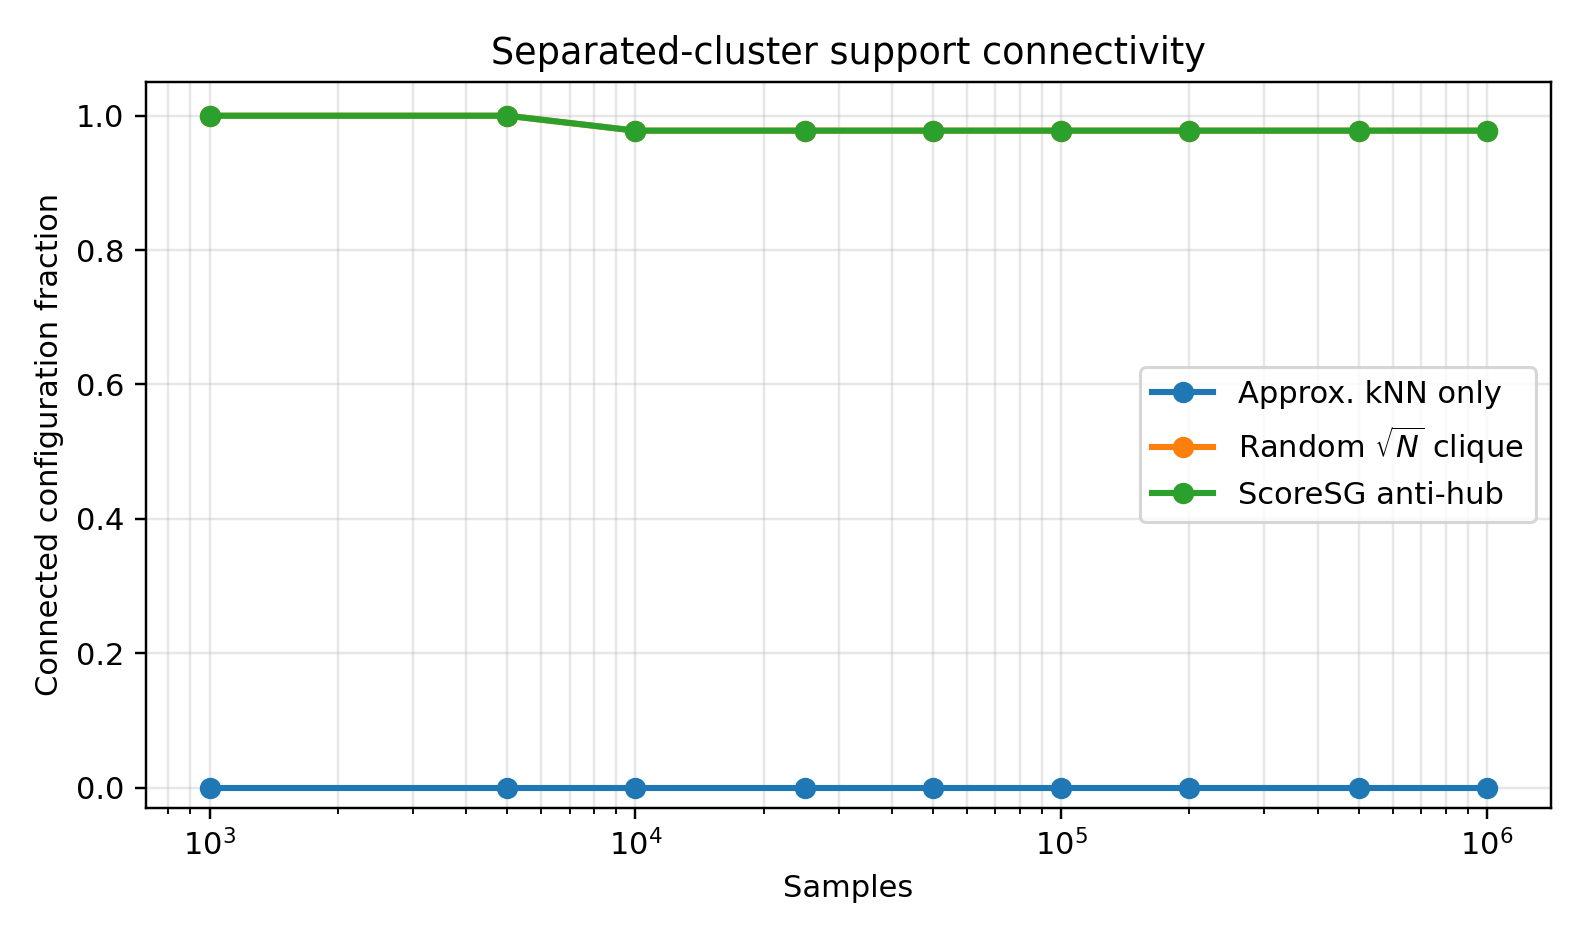
\includegraphics[width=0.82\linewidth,keepaspectratio]{missing_edges_connectivity_by_sample_size.png}
\caption{Connected-configuration fraction by sample size in the final separated-cluster support-graph diagnostic. Each point aggregates 45 configurations: nine distributions and five dimensions. The approximate \(k\)NN-only support is disconnected in every tested configuration, whereas both reinforced variants are connected in all configurations for \(N\in\{1{,}000,5{,}000\}\) and in 44 of 45 configurations for each larger sample size. Connectivity is necessary for MST extraction but does not certify complete-graph MST-edge recovery.}
\label{fig:connectivity-by-sample-size}
\end{figure}

The comparison with the random baseline changes the interpretation of this diagnostic. Relative to the approximate \(k\)NN-only support, both reinforced variants substantially improve connectivity in separated synthetic clusters. However, the random baseline and ScoreSG are indistinguishable on this binary connectivity metric in the final grid: both connect 398 of 405 configurations and fail on the same seven Poisson \(d=2\) cases. This does not imply that random selection recovers the same missing edges as anti-hub selection. Missing edges are the complete-graph MST edges absent from the approximate \(k\)NN support, and connectivity does not identify which MST edges are present. The present experiment therefore supports sparse clique reinforcement as a useful structural repair mechanism, but it does not demonstrate that anti-hub selection is superior to random selection on connectivity alone.

\section{Datasets and Experimental Setup}
\label{sec:experimental-setup}

\subsection{Synthetic Datasets}

The experimental evaluation uses synthetic datasets only. The runtime benchmark uses Gaussian-mixture data generated with \texttt{sklearn.datasets.make\_blobs}. This setting isolates runtime scaling with respect to \(N\) while holding the dimension, number of centers, and distance metric fixed. The common runtime comparison uses \(N \in \{5{,}000,10{,}000,20{,}000,30{,}000,40{,}000,50{,}000\}\), 20 features, 10 centers, and 30 timing repetitions per configuration; the ScoreSG-only scaling experiment extends to \(N=200{,}000\).

The quality benchmark uses a Gaussian synthetic grid with two dataset structures: IID Gaussian samples and separated Gaussian clusters with six generated centers. The tested sample sizes are \(N \in \{5{,}000,10{,}000,20{,}000,30{,}000,40{,}000\}\), the feature dimensions are \(d \in \{2,10,32,64\}\), and the dataset seed is 1. This produces 40 dataset configurations: one distribution, two structures, five sample sizes, four dimensions, and one seed. Table~\ref{tab:data} summarizes the dataset configurations used in the runtime and quality experiments.

\begin{table}[H]
\centering
\caption{Synthetic dataset configurations used in the experiments. The evaluation is unsupervised; train/validation/test splits are therefore not part of the protocol.}
\label{tab:data}
\resizebox{\linewidth}{!}{
\begin{tabular}{p{0.25\linewidth}p{0.32\linewidth}p{0.32\linewidth}}
\toprule
Setting & Runtime benchmark & Quality benchmark \\
\midrule
Generator & \texttt{make\_blobs} & \texttt{make\_synthetic\_distribution} and separated-cluster generator \\
Distributions & Gaussian blobs & \texttt{gaussian} \\
Dataset structures & Separated Gaussian mixture & IID synthetic samples; separated synthetic clusters \\
Samples & 5k, 10k, 20k, 30k, 40k, 50k; ScoreSG-only scaling to 200k & 5k, 10k, 20k, 30k, 40k \\
Features & 20 & 2, 10, 32, 64 \\
Centers & 10 & 6 for separated-cluster datasets; not applicable to IID datasets \\
Seeds & 30 timing repetitions per configuration & Dataset seed 1 \\
Metric & Euclidean & Euclidean \\
Total dataset configurations & 6 common runtime sample sizes; 12 ScoreSG-only scaling sizes & 40 synthetic configurations: 1 distribution \(\times\) 2 structures \(\times\) 5 sample sizes \(\times\) 4 dimensions \(\times\) 1 seed \\
\bottomrule
\end{tabular}
}
\end{table}

\subsection{Compared Methods}

Four methods are evaluated in the common comparison.
\begin{itemize}[leftmargin=*]
  \item \textbf{ScoreSG}: the proposed approximate anti-hub-reinforced construction, using optimized extraction.
  \item \textbf{CoreSG}: the exact reusable-support baseline introduced for multiple density-based MSTs \citep{araujo2022coresg}, using optimized extraction.
  \item \textbf{Optimized HDBSCAN}: the scikit-learn-contrib HDBSCAN implementation associated with Leland McInnes and collaborators, using \texttt{algorithm="best"} so that the implementation selects its optimized internal strategy \citep{mcinnes2017accelerated,hdbscansoftware}.
  \item \textbf{HDBSCAN}: the same HDBSCAN formulation executed with the generic internal algorithm, included to measure the cost of the non-specialized execution path.
\end{itemize}

For Optimized HDBSCAN and HDBSCAN, \texttt{min\_cluster\_size=k}, \texttt{min\_samples=k}, \texttt{approx\_min\_span\_tree=False}, and \texttt{gen\_min\_span\_tree=True}. For ScoreSG and CoreSG, the graph is built once at \(k_{\max}=50\), and hierarchies are extracted for \(k=50,49,\ldots,2\). This produces 49 requested hierarchy outputs per dataset configuration. Runtime configurations are repeated 30 times for timing stability, whereas the quality benchmark uses one execution for each dataset configuration in Table~\ref{tab:data}.

\subsection{Evaluation Metrics}

The primary metric reported in this version is cumulative wall-clock runtime for all 49 requested \(k\) values. This metric matches the target use case: repeated multi-resolution hierarchy extraction from a fixed dataset. For ScoreSG and CoreSG, cumulative runtime is computed as one construction at \(k_{\max}\) plus the sum of the 49 extraction times. For Optimized HDBSCAN and HDBSCAN, cumulative runtime is the sum of 49 independent executions, one for each value of \(k\).

The quality metrics are Adjusted Rand Index (ARI) \citep{hubert1985comparing} and Hierarchy Agreement Index (HAI) \citep{johnson2013comprehensive}. ARI is computed for each value of \(k\). For all quality configurations, ARI is computed against HDBSCAN with the generic internal algorithm, which serves as the reference implementation. For separated-cluster datasets, ARI is also computed against the generator labels.

HAI compares two hierarchies \(H_a\) and \(H_b\) over the same \(N\) objects. Let \(s_H(i,j)\) denote the size of the smallest cluster in hierarchy \(H\) that contains both objects \(x_i\) and \(x_j\), normalized by \(N\). We compute HAI as
\begin{equation}
  \mathrm{HAI}(H_a,H_b)
  =
  1 -
  \frac{2}{N^2}
  \sum_{1 \leq i < j \leq N}
  \left|s_{H_a}(i,j) - s_{H_b}(i,j)\right|.
\end{equation}
Thus, \(\mathrm{HAI}=1\) indicates identical pairwise hierarchy structure under this representation, whereas lower values indicate larger differences in the levels at which point pairs merge. In our protocol, HAI compares the hierarchy produced by each method against the hierarchy produced by HDBSCAN with the generic internal algorithm for the same dataset and \(k\) sequence.

All wall-clock timings are reported for the local benchmark environment used in this study. Consequently, the absolute seconds should be interpreted as measurements for that environment, while relative growth patterns and within-environment comparisons are the main object of analysis.

\section{Results}
\label{sec:results}

\subsection{Runtime Evaluation: Cumulative Multi-k Cost}

Table~\ref{tab:mainresults} and Figure~\ref{fig:runtime-common} report cumulative runtime for the common comparison interval. Each number represents the total cost of obtaining 49 results for \(k=50,49,\ldots,2\). This accumulation is the central performance object: the expected workflow is not a single clustering run, but the inspection of a sequence of density resolutions over the same data.

\begin{table}[H]
\centering
\caption{Cumulative runtime in seconds for the 49-value multi-\(k\) workflow. Values are means with cumulative standard deviations aggregated from 30 timing repetitions for each requested \(k\).}
\label{tab:mainresults}
\resizebox{\linewidth}{!}{
\begin{tabular}{lrrrrrr}
\toprule
Method & 5k & 10k & 20k & 30k & 40k & 50k \\
\midrule
ScoreSG & \textbf{12.69 \(\pm\) 0.04} & \textbf{28.44 \(\pm\) 0.04} & \textbf{65.10 \(\pm\) 0.06} & \textbf{111.28 \(\pm\) 0.11} & \textbf{166.37 \(\pm\) 0.48} & \textbf{224.36 \(\pm\) 0.71} \\
CoreSG & 14.29 \(\pm\) 0.03 & 36.11 \(\pm\) 0.04 & 100.21 \(\pm\) 0.16 & 191.72 \(\pm\) 0.49 & 381.33 \(\pm\) 24.86 & 525.45 \(\pm\) 34.21 \\
Optimized HDBSCAN & 35.43 \(\pm\) 0.04 & 91.22 \(\pm\) 0.08 & 331.03 \(\pm\) 0.54 & 542.19 \(\pm\) 0.65 & 980.50 \(\pm\) 10.10 & 1342.44 \(\pm\) 16.98 \\
HDBSCAN & 76.68 \(\pm\) 0.05 & 299.81 \(\pm\) 0.26 & 1429.84 \(\pm\) 30.68 & 2894.76 \(\pm\) 3.89 & 6747.33 \(\pm\) 17.73 & 9272.92 \(\pm\) 23.85 \\
\bottomrule
\end{tabular}
}
\end{table}

\begin{figure}[H]
\centering
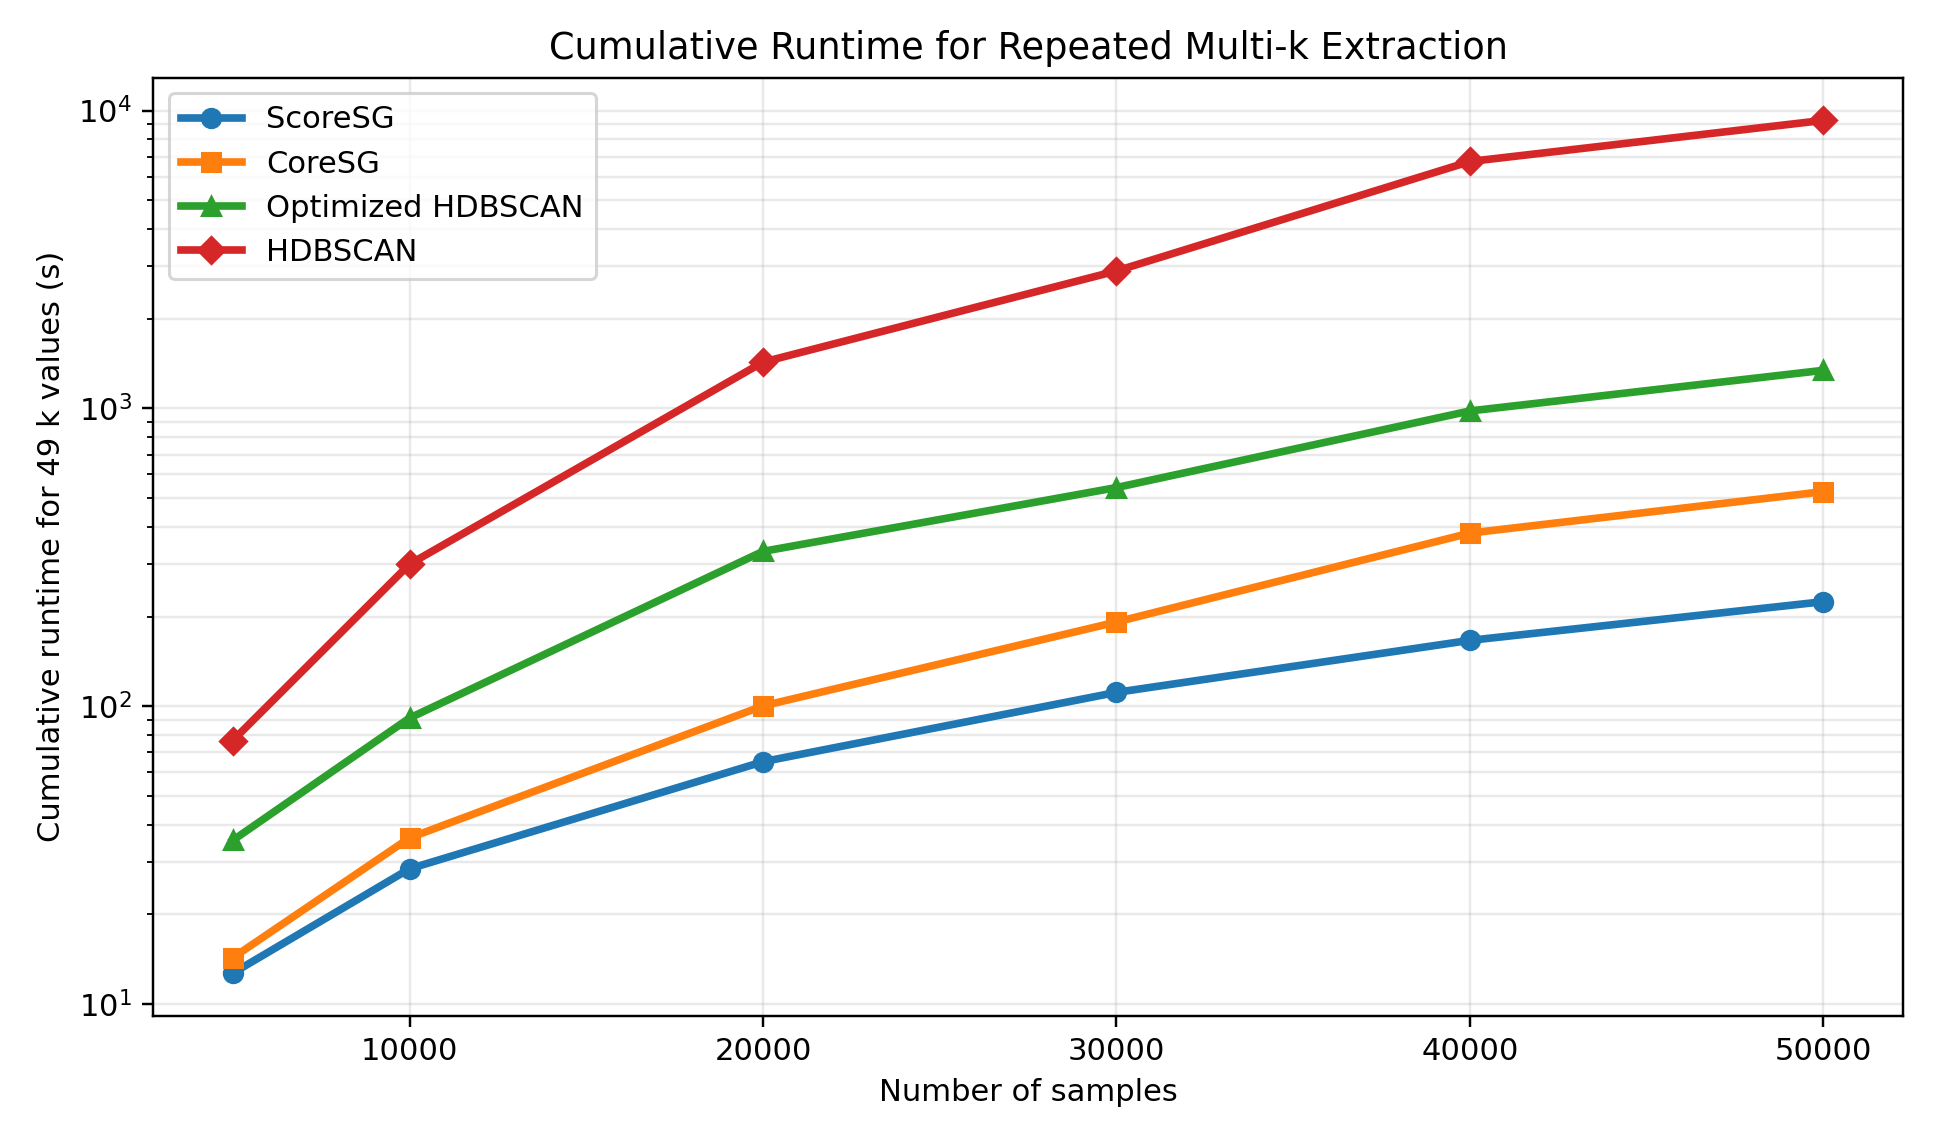
\includegraphics[width=\linewidth,keepaspectratio]{score_sg_common_runtime.png}
\caption{Cumulative runtime on the common comparison interval. The y-axis uses a logarithmic scale. ScoreSG remains below CoreSG, Optimized HDBSCAN, and HDBSCAN across all tested sample sizes.}
\label{fig:runtime-common}
\end{figure}

At \(N=50{,}000\), ScoreSG requires 224.36 s for all \(k\) values. CoreSG requires 525.45 s, Optimized HDBSCAN requires 1342.44 s, and HDBSCAN requires 9272.92 s. Thus, the observed speedups of ScoreSG are \(2.34\times\), \(5.98\times\), and \(41.33\times\), respectively. The advantage over CoreSG shows that the approximate anti-hub support graph reduces the cost of the reusable strategy itself. The larger gap relative to Optimized HDBSCAN and HDBSCAN reflects the cost of recomputing the hierarchy 49 times instead of reusing a constructed support graph.

\subsection{Scalability Beyond the Common Comparison}

The main scalability question is whether the sparse construction continues to support larger sample sizes after exact dense construction becomes increasingly expensive. Figure~\ref{fig:runtime-extended} reports ScoreSG scaling up to \(N=200{,}000\). Because corresponding CoreSG and HDBSCAN measurements are not available beyond \(N=50{,}000\), this experiment evaluates ScoreSG's internal scaling rather than comparative superiority over the extended range.

\begin{figure}[H]
\centering
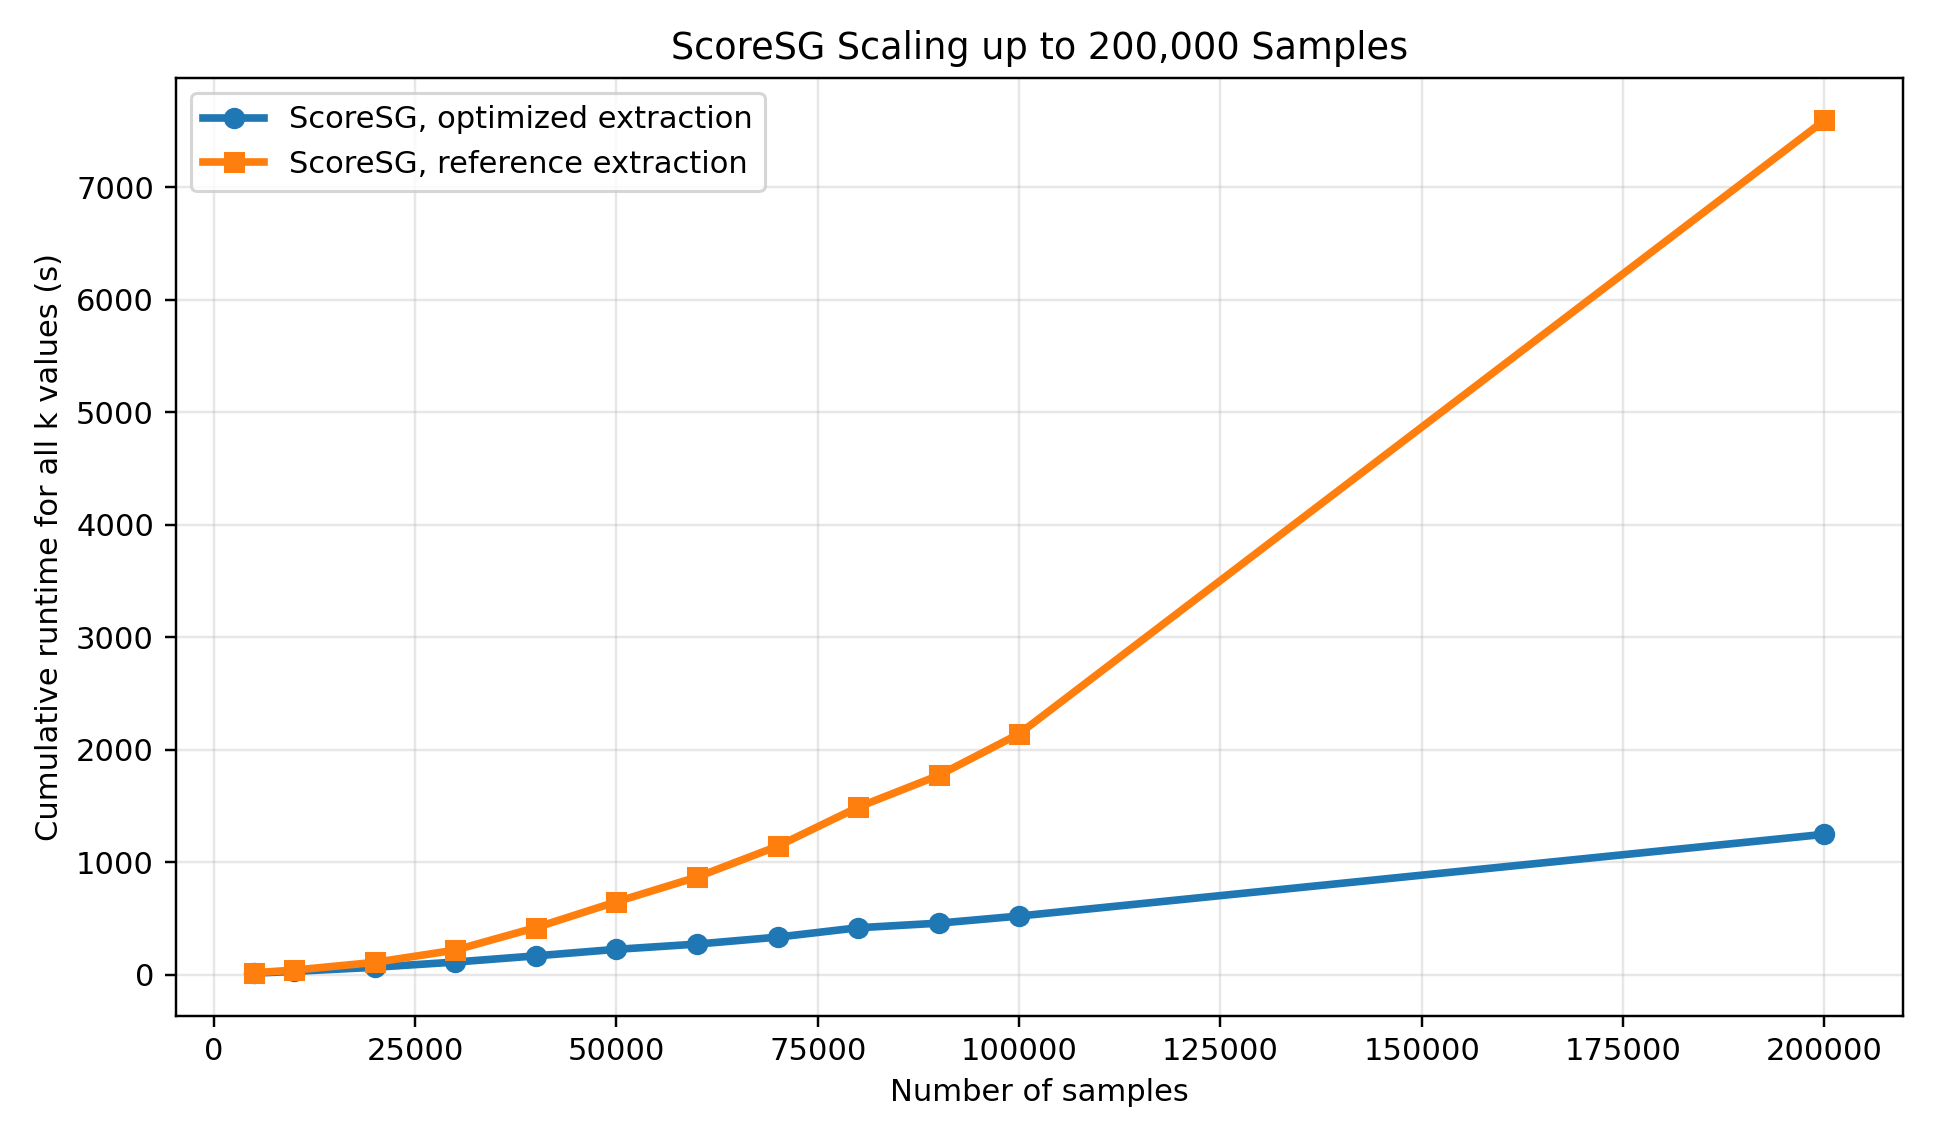
\includegraphics[width=\linewidth,keepaspectratio]{score_sg_extended_runtime.png}
\caption{ScoreSG cumulative runtime scaling up to \(N=200{,}000\). Optimized extraction grows substantially more slowly than the reference extraction path, indicating that sparse construction alone is insufficient without efficient repeated extraction.}
\label{fig:runtime-extended}
\end{figure}

The optimized ScoreSG implementation increases from 12.69 s at \(N=5{,}000\) to 1246.93 s at \(N=200{,}000\). A log-log fit over these measurements gives an empirical exponent of approximately 1.26 for optimized ScoreSG. This exponent is a descriptive scaling summary over the measured interval, not an asymptotic proof. The reference extraction path grows more rapidly and reaches 7592.37 s at \(N=200{,}000\), indicating that extraction optimization is an essential part of the observed scalability. The separation between the two ScoreSG curves also indicates that sparse construction alone is not sufficient: scalable multi-\(k\) analysis requires both a sparse support graph and efficient repeated extraction from that support.

\subsection{Quality Evaluation: ARI and HAI}

Runtime is only one axis of evaluation. Because ScoreSG is approximate, the benchmark must evaluate both clustering partitions and hierarchy fidelity. ARI measures agreement between predicted labels and either synthetic generator labels or labels from an exact reference method. HAI measures pairwise agreement between hierarchy structures by comparing the normalized size of the smallest shared cluster for every point pair \citep{johnson2013comprehensive}. Table~\ref{tab:quality-layout} reports the aggregate quality results over the Gaussian synthetic quality grid.

\begin{table}[H]
\centering
\caption{Quality results for the Gaussian synthetic benchmark. Values aggregate 40 dataset configurations and 1960 requested \(k\) evaluations per method. ARI-ref is computed against HDBSCAN with the generic internal algorithm. ARI-true is computed only for separated-cluster datasets, where generator labels are available. Workflow time is the mean cumulative time, in seconds, over the 49-value multi-\(k\) sequence.}
\label{tab:quality-layout}
\resizebox{\linewidth}{!}{
\begin{tabular}{lrrrrrrrr}
\toprule
Method & Successful \(k\) & Mean ARI-ref & Min. ARI-ref & Mean ARI-true & Min. ARI-true & Mean HAI & Min. HAI & Mean workflow time \\
\midrule
HDBSCAN & 1960/1960 & 1.0000 & 1.0000 & 0.9905 & 0.0011 & 1.0000 & 1.0000 & 1482.21 \\
Optimized HDBSCAN & 1960/1960 & 0.9999 & 0.9654 & 0.9905 & 0.0011 & 1.0000 & 1.0000 & 1163.10 \\
ScoreSG & 1960/1960 & 0.9015 & -0.1452 & 0.9999 & 0.9010 & 0.9738 & 0.8333 & 87.70 \\
ScoreSG Random & 1960/1960 & 0.9015 & -0.1452 & 0.9999 & 0.9010 & 0.9530 & 0.7593 & 86.83 \\
\bottomrule
\end{tabular}
}
\end{table}

All four methods complete all requested \(k\) evaluations in the quality benchmark. ScoreSG has a mean workflow time of 87.70 s, which is \(16.90\times\) faster than generic HDBSCAN and \(13.26\times\) faster than Optimized HDBSCAN on this grid. ScoreSG Random has nearly the same runtime, with a mean workflow time of 86.83 s.

Against the generic HDBSCAN reference, ScoreSG obtains mean ARI 0.9015 and mean HAI 0.9738. The negative minimum ARI indicates that some individual \(k\) values or dataset configurations diverge strongly from the HDBSCAN reference partition. However, on the separated-cluster datasets where generator labels are available, ScoreSG obtains mean ARI-true 0.9999 and minimum ARI-true 0.9010. This contrast indicates that disagreement with HDBSCAN does not necessarily imply poor recovery of the generated cluster structure in the separated synthetic setting.

The comparison between ScoreSG and ScoreSG Random is informative. The two methods have the same aggregate ARI values against HDBSCAN and nearly identical ARI values against the generator labels, but ScoreSG has higher hierarchy agreement: mean HAI 0.9738 versus 0.9530, and minimum HAI 0.8333 versus 0.7593. Thus, in this quality benchmark, anti-hub selection improves hierarchy fidelity relative to random sparse clique reinforcement even when flat partition agreement is essentially unchanged.

\section{Discussion}
\label{sec:discussion}

\subsection{Connectivity and Missing-Edge Recovery}

The connectivity diagnostics clarify the structural role of sparse reinforcement before runtime is considered. In the final separated-cluster stress test, the approximate \(k\)NN-only support was disconnected in every evaluated configuration, whereas both reinforced variants were connected in 398 of 405 configurations. This result supports the claim that adding a linear-size reinforcement clique can repair the minimum connectivity condition in most compact, well-separated synthetic clusters. It does not support the stronger claim that anti-hub ranking is better than random vertex selection for connectivity alone: the random \(\sqrt{N}\)-clique baseline and ScoreSG produced identical connected-configuration counts and failed on the same Poisson \(d=2\) settings. The result also illustrates why connectivity cannot be used as a proxy for missing-edge recovery: a connected graph may still omit complete-graph MST edges, and a randomly repaired graph may connect components without preserving the hierarchy induced by mutual-reachability distances. The anti-hub mechanism remains motivated by the low in-degree missing-support hypothesis and by its deterministic tie-aware ranking, but its advantage must be evaluated with stricter criteria such as MST edge recall, HAI, ARI, and stability across seeds.

\subsection{Runtime and Workflow Implications}

The runtime results indicate that, when the support graph is usable, ScoreSG changes the cumulative performance profile of repeated HDBSCAN-style hierarchy extraction. The improvement is consistent with the method design: dense pairwise construction is replaced by sparse approximate support, while the reusable CoreSG extraction principle avoids rerunning HDBSCAN independently for every \(k\). Optimized HDBSCAN is a strong practical baseline because it uses optimized internal algorithm selection, but it still pays the cost of a full fit for each requested parameter value.

\subsection{Quality Evidence}

The quality results clarify the scope of the approximation. ScoreSG is much faster than both HDBSCAN baselines in the Gaussian quality grid and preserves high average hierarchy agreement with the generic HDBSCAN reference. However, the negative minimum ARI-ref shows that flat partitions can still diverge substantially for some individual configurations or \(k\) values. Approximate neighbor errors can change core-distance estimates; missing support edges can alter MST structure; and both random and anti-hub clique edges can affect hierarchy topology. Therefore, the present findings justify ScoreSG as a scalable computational method with strong average quality behavior on the tested Gaussian synthetic grid, not as a universally equivalent approximation of exact HDBSCAN or exact CoreSG.

\subsection{Limitations}

The evaluation has five main limitations. First, all reported datasets are synthetic. The runtime benchmark uses Gaussian mixtures with fixed dimension, number of centers, and dataset seed, while the quality benchmark uses a Gaussian grid with seed 1. Second, the broader connectivity diagnostic covers nine distributions, separated-cluster synthetic geometries, sample sizes from \(10^3\) to \(10^6\), and dimensions from 2 to 128, but it measures connectivity rather than direct MST-edge recall. Third, the common runtime comparison with CoreSG, Optimized HDBSCAN, and HDBSCAN ends at \(N=50{,}000\); results beyond that point are ScoreSG-only. Fourth, the reported wall-clock times characterize one benchmark environment, so absolute seconds may differ on other hardware or software stacks. Fifth, anti-hub reinforcement is a heuristic and does not prove recovery of all complete-graph MST edges; in the connectivity diagnostic, it also does not outperform a random \(\sqrt{N}\)-clique baseline on the binary connectivity metric. The random baseline result must be interpreted only as a connectivity result, not as evidence that random reinforcement preserves missing MST edges or clustering quality.

\section{Ethics and Broader Impact}

The reported experiments use synthetic data and do not include personal or sensitive attributes. Privacy and consent risks are therefore minimal for the benchmark itself. However, density-based clustering can be used for customer segmentation, anomaly detection, profiling, and operational decision support. Deployments involving people require separate analysis of consent, sensitive attributes, fairness, privacy, and downstream harms. The present paper does not provide evidence for use in high-stakes decision systems.

The environmental impact of the reported benchmark is limited by the scale of the experiments, but larger repeated clustering workflows can consume substantial compute. ScoreSG may reduce energy use in exploratory multi-\(k\) workflows by reducing repeated computation; direct energy consumption was not measured in this study.

\section{Conclusion}

ScoreSG is a sparse approximate support-graph construction method for repeated multi-\(k\) density hierarchy extraction. It combines approximate neighbor discovery with anti-hub reinforcement and reuses the CoreSG MST and hierarchy pipeline. The connectivity diagnostic shows that the ScoreSG support graph was connected in 398 of 405 separated-cluster synthetic configurations, while the approximate \(k\)NN-only support was connected in 0 of 405. A random \(\sqrt{N}\)-clique baseline was also connected in 398 of 405 configurations, so connectivity alone does not establish superiority of anti-hub selection. More importantly, connectivity does not imply recovery of missing edges, because missing edges are the complete-graph MST edges absent from the approximate \(k\)NN support. In the tested synthetic runtime benchmark, ScoreSG has the lowest cumulative runtime across all common sample sizes and achieves a \(5.98\times\) observed speedup over Optimized HDBSCAN at \(N=50{,}000\). In the Gaussian quality benchmark, ScoreSG completed all 1960 requested \(k\) evaluations, with mean ARI-ref 0.9015, mean HAI 0.9738, and mean workflow time 87.70 s.

The conclusion is therefore limited but concrete: ScoreSG improves cumulative runtime in repeated multi-\(k\) workflows, often repairs the minimum connectivity condition required for MST extraction, and preserves high average hierarchy agreement with the HDBSCAN reference on the tested Gaussian quality grid. Future work should extend the quality benchmark to additional distributions, evaluate direct MST-edge recall, analyze the configurations with low ARI-ref, and profile memory use. A multi-GPU ScoreSG implementation is also a concrete next step, because approximate neighbor construction and repeated extraction are both natural targets for parallel acceleration at larger scale.

\section*{Code Availability}

ScoreSG is implemented in the Python package \texttt{core-sg}, version 0.0.1, distributed under a BSD-3-Clause license \citep{coresgsoftware}. The package exposes ScoreSG through \texttt{CoreSG(algorithm="score-sg")} and the estimator-compatible interface in \texttt{CoreSGClusterer}.


\bibliographystyle{plainnat}
\bibliography{references}

\end{document}
